% Generated by code/draw_circuits.py.
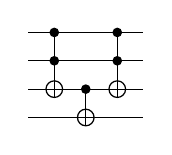
\begin{tikzpicture}[x=1cm,y=1cm,baseline={([yshift=-0.25em]mid)},line width=.45pt]
\coordinate (mid) at (0,-0.540);
\draw (0,0.000)--(1.460,0.000);
\draw (0,-0.360)--(1.460,-0.360);
\draw (0,-0.720)--(1.460,-0.720);
\draw (0,-1.080)--(1.460,-1.080);
\draw (0.330,0.000)--(0.330,-0.720);
\filldraw[fill=black] (0.330,0.000) circle[radius=1.5pt];
\filldraw[fill=black] (0.330,-0.360) circle[radius=1.5pt];
\draw[fill=white] (0.330,-0.720) circle[radius=3pt];
\draw (0.225,-0.720)--(0.435,-0.720) (0.330,-0.825)--(0.330,-0.615);
\draw (0.730,-0.720)--(0.730,-1.080);
\filldraw[fill=black] (0.730,-0.720) circle[radius=1.5pt];
\draw[fill=white] (0.730,-1.080) circle[radius=3pt];
\draw (0.625,-1.080)--(0.835,-1.080) (0.730,-1.185)--(0.730,-0.975);
\draw (1.130,0.000)--(1.130,-0.720);
\filldraw[fill=black] (1.130,0.000) circle[radius=1.5pt];
\filldraw[fill=black] (1.130,-0.360) circle[radius=1.5pt];
\draw[fill=white] (1.130,-0.720) circle[radius=3pt];
\draw (1.025,-0.720)--(1.235,-0.720) (1.130,-0.825)--(1.130,-0.615);
\end{tikzpicture}
